\documentclass[11pt,a4paper,xcolor=table]{beamer} % ,handout: for printing
\usepackage{etex}
%\documentclass[handout]{beamer}

\usetheme{Madrid}

%
% To use when printing
%
\iffalse
\usepackage{pgfpages}
\mode<handout>{
  \usetheme{default}
  \setbeamercolor{}{bg=black!5} % \setbeamercolor{background canvas}{bg=black!5} 
  \pgfpagesuselayout{4 on 1}[letterpaper,landscape,border shrink=2.5mm]
}
\fi

\usepackage[utf8]{inputenc} % [utf8] for linux, latin1 for windows
\usepackage[french]{babel}
%\usepackage{fullpage}
\usepackage{amsmath}
\usepackage{amsfonts}
\usepackage{amssymb}
\usepackage{graphicx} 
\usepackage{longtable}
\usepackage{algorithm}
\usepackage{listings}
\usepackage{algorithmic}
\usepackage{float}

\usepackage[center]{caption}
\usepackage{subcaption}

\usepackage[table]{xcolor}

\definecolor{colorperso}{RGB}{165,165,165}
%\usepackage[utf8]{inputenc}
%\usepackage[francais]{babel}
%\usepackage[T1]{fontenc}

%\usepackage{amsmath}
%\usepackage{amsfonts}
%\usepackage{amssymb}

%\usepackage{amsthm}
%\usepackage{graphicx}

\usepackage{tikz,pgfplots}
\usepackage[all]{xy}

% tikz stuff
\usetikzlibrary{shapes,arrows,decorations.pathreplacing, calc, intersections}
\makeatletter
\newcommand{\gettikzxy}[3]{%
  \tikz@scan@one@point\pgfutil@firstofone#1\relax
  \edef#2{\the\pgf@x}%
  \edef#3{\the\pgf@y}%
}
\makeatother

\newtheorem*{mydef}{Definition}
%\newtheorem*{definition}{Definition}
\newtheorem{mythm}{Theorem}
\newtheorem{requirement}{Requirement}
\newtheorem*{mynot}{Notation}
\newtheorem{myprop}{Proposition}

\newcommand{\var}{\operatorname{Var}}


\makeatother
\setbeamertemplate{footline}
{
  \leavevmode%
  \hbox{%
  \begin{beamercolorbox}[wd=.4\paperwidth,ht=2.25ex,dp=1ex,center]{author in head/foot}%
    \usebeamerfont{author in head/foot}\insertshortauthor
  \end{beamercolorbox}%
  \begin{beamercolorbox}[wd=.6\paperwidth,ht=2.25ex,dp=1ex,center]{title in head/foot}%
    \usebeamerfont{title in head/foot}\insertshorttitle\hspace*{3em}
    \insertframenumber{} / \inserttotalframenumber\hspace*{1ex}
  \end{beamercolorbox}}%
  \vskip0pt%
}
\makeatletter

\setbeamertemplate{navigation symbols}{}

\author[]{Jean-Baptiste Lespiau}
\author{Jean-Baptiste Lespiau et Charles Thin}
\title{La méthode B : une méthode formelle de développement logiciel}
\date\today

\begin{document}

\frame{\titlepage}

\section*{Introduction}

\begin{frame}
\frametitle{Introduction}
\framesubtitle{Qu'est-ce que la méthode B ?}
La méthode B, inventée par Jean-Raymond Abrial, c'est :\\~\\
\begin{itemize}
\pause
\item Un langage (le langage B)\\~\\
\pause
\item Un outil (l'Atelier B)\\~\\
\pause
\item Une méthode (la méthode B)
\end{itemize}
\end{frame}

\begin{frame}
\frametitle{Introduction}
\framesubtitle{À quoi sert ... le langage B ?}
B est un langage unique pour :\\~\\
\pause
\begin{itemize}
\item Spécifier formellement des fonctionnalités du logiciel
\pause
\item Spécifier formellement des propriétés du logiciel
\pause
\end{itemize}
~\\
Et ce à tout niveau d'abstraction.
\end{frame}

\begin{frame}
\frametitle{Introduction}
\framesubtitle{À quoi sert ... l'Atelier B ?}
\begin{figure}[h]
\centering

\includegraphics[scale=0.33]{ressources/logo.png}
\end{figure}
L'Atelier B (ClearSy) est l'outil principal où l'on écrit du B et où on le vérifie. Il est donc au coeur de la méthode B.\\~\\
\pause
Il comprend :
\begin{itemize}
\item un analyseur
\pause
\item un générateur d'obligation de preuve
\pause
\item un démonstrateur automatique
\pause
\item un démonstrateur interactif
\pause
\item un générateur de code C et Ada
\pause
\item un gestionnaire de projet...
\end{itemize}
\end{frame}

\begin{frame}
\frametitle{Introduction}
\framesubtitle{À quoi sert ... la méthode B ?}
\begin{figure}[h]
\centering

\includegraphics[scale=0.33]{ressources/logo1.png}
\end{figure}
La méthode B, enfin, encadre le processus industriel.\\~\\~\pause
C'est une méthode formelle par laquelle on peut :\pause
\begin{itemize}
\item Énoncer en B les fonctionnalité du logiciel en développement
\pause
\item Les raffiner (concrétiser) jusqu'à obtenir une implémentation
\pause
\end{itemize}
Et en même temps :\pause
\begin{itemize}
\item Énoncer en B des propriétés sur le logiciel en développement
\pause
\item Les vérifier lors du développement (du raffinement) dans l'Atelier B
\pause
\end{itemize}
Pour enfin :
\begin{itemize}
\item Générer du code fonctionnel (en un langage compilable ``classique'') ...
\pause
\item ... qui vérifie par construction les propriétés voulues !
\end{itemize}
\end{frame}


\begin{frame}
\frametitle{Introduction} \iffalse TODO Introduction ? Ou plus tard ? \fi
\framesubtitle{Cycle de développement formel vs cycle conventionnel}
\begin{figure}[h]
\centering
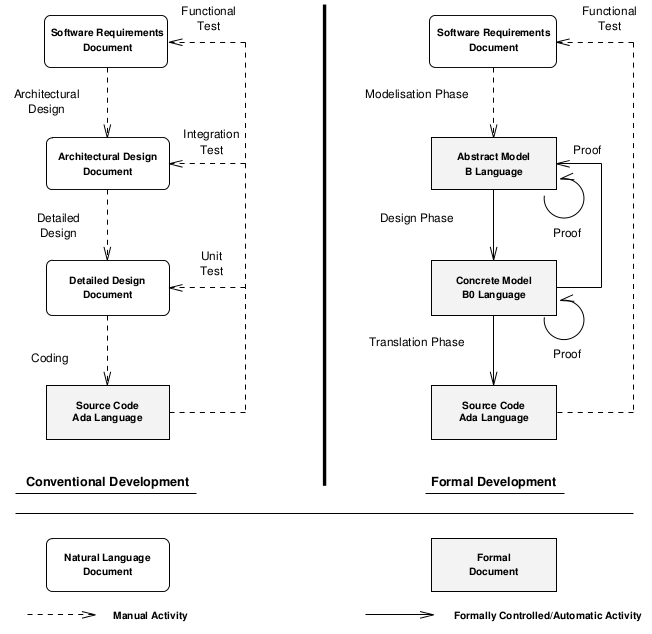
\includegraphics[scale=0.33]{ressources/formal_dev.png}
\end{figure}
\end{frame}

%
% Plan
%
\frame{\tableofcontents}

\section{Modélisation formelle}
\subsection{Théorie des ensembles}
\begin{frame}
\frametitle{Modélisation formelle}
\framesubtitle{Théorie des ensembles}
\begin{description}
\item[Définition de la paire] $(E, F) \in s \times t \Leftrightarrow E \in s \wedge F \in t$
\item[Ensemble des parties] $s \in \mathbb{P}(t) \Leftrightarrow \forall x (x \in s \Rightarrow x \in t)$
\item[Ensemble en compréhension] $E \in \{ x | x \in s \wedge P \} \Leftrightarrow (E \in s \wedge [x:= E] P)$
\item[Égalité d'ensembles] $\forall x (x \in s \Leftrightarrow x \in t) \Rightarrow s = t$
\item[Axiome du choix] $\exists x  (x \in s) \Rightarrow choice(s) \in s$
\item[Axiome de l'infini] Existence d'un ensemble infini nommé BIG
\end{description}
\end{frame}

\begin{frame}
\frametitle{Ce qu'il faut retenir}
\begin{itemize}
\item B est un langage et une méthode de spécification
\item C'est une méthode formelle (permettant des preuves)
\item Le langage est basé sur la théorie des ensembles
\item Une spécification simple est une machine abstraite
\item Une machine abstraite décrit :
\begin{itemize}
\item L'état du système modélisé (variables typées)
\item Certaines de ses propriétés (invariant)
\item Les services qu'il offre (opérations)
\end{itemize}
\item La vérification (preuve) assure que les services satisfont les
propriétés
\item Les preuves démontrent la préservation d'un invariant
\item Les preuves s'effectuent par calcul des plus faibles préconditions
(calcul des substitutions)
\end{itemize}
\end{frame}

\section{Modélisation en méthode B}
\subsection{Les machines abstraites}
\begin{frame}
\frametitle{Les machines abstraites}
\framesubtitle{Un exemple}

\end{frame}

\subsection{Le raffinement de machines}
\begin{frame}
\frametitle{Le raffinement de machines}
Le raffinement est le fait de transformer une spécification abstraite en un texte plus proche de la programmation, pour finalement obtenir un programme.

En pratique il s'agit de :
\begin{itemize}
\item Reformulation en fonction du changement d’état
\item Affaiblissement des préconditions
\item Réduction du non-déterminisme
\end{itemize}

\end{frame}



\subsection{L'implémentation}
\begin{frame}
\frametitle{Implémentations}
Le langage $B_0$ est un sous langage de la méthode B qui est directement traduisible en un programme (en ADA, C, C++, etc.).  Il est ainsi très proche d'un langage séquentiel.

\pause

On impose un certain nombre de restrictions :
\begin{itemize}
\item aucune précondition
\item que des substitutions déterministes ( $:=$, \textsc{IF}, ";" par exemple)
\item toutes les constantes et variables sont d'un type concret
\item la terminaison et la correction des boucles doit être prouvée par l'utilisation d'invariants et de variants
\end{itemize}

\end{frame}

\begin{frame}
\frametitle{Implémentations}
\framesubtitle{Un exemple}
\end{frame}

\section{Preuve de propriétés}
\begin{frame}
\frametitle{Preuve de programmes}
Le système de preuve est basée sur la vérification que :
\begin{itemize}
\item Les propriétés invariantes sont vérifiées par la
dynamique
\item Les raffinements préservent la correction totale
des propriétés invariantes
\end{itemize}

\pause
Pour cela, on se base sur la logique de Hoare :
\begin{itemize}
\item
Principe de correction partielle : $ \{P\}\;S\;\{Q\} $ 

Si l'état satisfait P avant S et si S termine, alors l'état satisfait Q après l'exécution de S.
\item
Recherche de la plus faible précondition:

Si l'état satisfait wp(S, Q) avant S alors S termine et l'état satisfait Q après.
On le note sous la forme de la substitution $[S]Q$.
\end{itemize}
\end{frame}

\begin{frame}
En résumé, le processus de raffinage consiste à :
\begin{itemize}
\item réduire l'indéterminisme
\item affaiblir les préconditions
\item renforcer les gardes
\item s'approcher de la machine concrète avec introduction u séquencement et de la boucle
on prouve que le raffinage se fait en respectant les fonctionnalités
\end{itemize}
\end{frame}


\iffalse
\subsection{Raffinement}
\begin{frame}
\frametitle{Obligations de preuve}
\begin{columns}[t]
  \begin{column}{5cm}
    \textsc{machine} $M$ \\
    \textsc{variables} $x$ \\
    \textsc{invariant} $I$ \\
    \textsc{initialisation} $U$ \\
    \textsc{operations} \\
    \quad $r \longleftarrow nom\_op(w) =$ \\
    \qquad \textsc{pre} $P$ \textsc{then} $K$ \textsc{end} \\
    \textsc{end}
\end{column}
  
  \begin{column}{5cm}
    \textsc{refinement} $N$ \textsc{refines} $M$ \\
    \textsc{variables} $y$ \\
    \textsc{invariant} $J$ \\
    \textsc{initialisation} $V$ \\
    \textsc{operations} \\
    \quad $r \longleftarrow nom\_op(w) =$ \\
    \qquad \textsc{pre} $Q$ \textsc{then} $L$ \textsc{end} \\
    \textsc{end}  
  \end{column}
\end{columns}  
 
Pour chaque opération il faut prouver:
\begin{itemize}
\item I ∧ J ∧ P ⇒ Q 
\item 
\end{itemize}
\end{frame}
\fi

\section{Diffusion de la méthode B}
\begin{frame}
\frametitle{Diffusion de la méthode B}
\framesubtitle{Météor}
Logiciel sécuritaire : 86 000 lignes Ada (1 000
composants)
\begin{itemize}
\item 115 000 lignes B
\item 27 800 obligations de preuve
\begin{itemize}
\item 81\% de preuve automatique
\item 92\% après ajout de règles (550)
\item 2 254 à prouver interactivement
\end{itemize}
\item Utilisateur d'un matériel sûr Vital Coded Processor (VCP) : processeur vérifiant son état et l'intégrité du code exécuté
\end{itemize}
\end{frame}

\begin{frame}
\frametitle{La méthode B événementielle}

\end{frame}

\end{document}